% thanks to ChatGPT and Claude

\documentclass{standalone}
\usepackage{tikz}
\usepackage{amsmath,amssymb}

\begin{document}
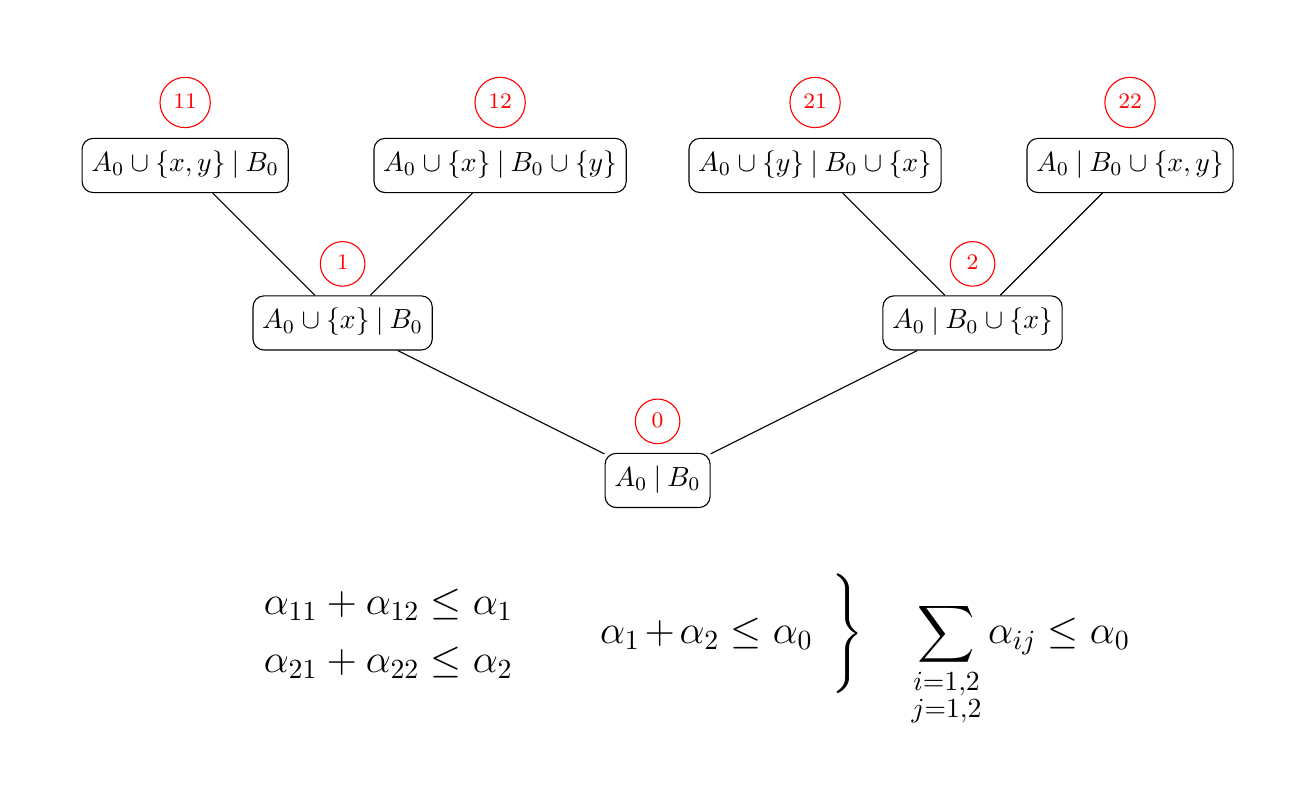
\begin{tikzpicture}[
    every node/.style={draw, rounded corners, text depth=1ex, text height=2ex},
    label/.style={red, draw, circle, font=\footnotesize, inner sep=1pt, minimum size=15pt}
]
% Set manual bounding box
\useasboundingbox (-8,-3.75) rectangle (8,5.75);

% Tree structure
\node (bottom) at (0,0) {$A_0 \mathbin{|} B_0$};
\node[label] at (0,0.75) {0};

\node (left) at (-4,2) {$A_0 \cup \{x\} \mathbin{|} B_0$};
\node[label] at (-4,2.75) {1};

\node (right) at (4,2) {$A_0 \mathbin{|} B_0 \cup \{x\}$};
\node[label] at (4,2.75) {2};

\node (ll) at (-6,4) {$A_0 \cup \{x,y\} \mathbin{|} B_0$};
\node[label] at (-6,4.8) {11};

\node (lr) at (-2,4) {$A_0 \cup \{x\} \mathbin{|} B_0 \cup \{y\}$};
\node[label] at (-2,4.8) {12};

\node (rl) at (2,4) {$A_0 \cup \{y\} \mathbin{|} B_0 \cup \{x\}$};
\node[label] at (2,4.8) {21};

\node (rr) at (6,4) {$A_0 \mathbin{|} B_0 \cup \{x,y\}$};
\node[label] at (6,4.8) {22};

% Connections
\draw (bottom) -- (left);
\draw (bottom) -- (right);
\draw (left) -- (ll);
\draw (left) -- (lr);
\draw (right) -- (rl);
\draw (right) -- (rr);

% Equations at the bottom
\node[draw=none, text width=11cm] at (0.5,-2) {
    \Large
    $\begin{alignedat}{2}
        \alpha_{11} &+ \alpha_{12} &{}\leq \alpha_1 \\
        \alpha_{21} &+ \alpha_{22} &{}\leq \alpha_2
    \end{alignedat}$
    \qquad
        $\alpha_{1} + \alpha_{2} \leq \alpha_0$
    \ \Bigg\}
    \quad
        $\displaystyle \sum_{\substack{i=1,2\\j=1,2}} \alpha_{ij} \leq \alpha_0$
};

\end{tikzpicture}
\end{document}